\nocite{*} % cargar toda la bib
  \begin{abstract}
    La extinción de especies de animales en la actualidad genera impactos variados para el medio ambiente, desde la aparición de plagas hasta el desequilibrio ambiental. Uno de los grandes problemas que existen en la actualidad es la desaparición de depredadores tope el cual debido a su ausencia, el ecosistema donde residía tuvo un aumento de población de otras especies llegando a valores extremos y provocando el cambio del mismo. Ante esto se buscó resolver esta problemática a través de una técnica llamada ``Rewilding'' que consiste en la inserción de individuos provenientes de otras zonas en el ambiente donde estaba extinto para que este vuelva a poblar su lugar. Esto podría traer beneficios desde ambientales hasta la posibilidad de creación de parques turísticos donde la población de personas podría aprovechar esta oportunidad y crear una economía basada en el atractivo de la especie.
    En el presente estudio se buscará aplicar esta técnica con la especie animal conocida como Yaguareté o Jaguar el cual se encontraba extinto en los Esteros del Iberá (correspondiente a la provincia de Corrientes), cuyo trabajo de reinserción se está realizando actualmente. La idea principal del modelo de simulación es analizar el crecimiento de la población de esta especie según distintas variables, recreando zonas con distintas características que analizaremos en las siguientes secciones.
    De cada zona en estudio se analizará el comportamiento de cada individuo al cazar, reproducirse, territorialidad de individuos y crecimiento de las crías.

  \end{abstract}

    \keywords{rewilding \and yaguareté \and jaguar \and ambiente \and simulación \and iberá \and felinos \and animales \and ecosistema \and biología \and puma \and medioambiente}

\newpage
\tableofcontents
\newpage

\section{Definición de sistema bajo estudio}
    Actualmente la población del yaguareté en la Argentina cuenta con aproximadamente 250 ejemplares, los cuales están distribuidos en distintas zonas del país. Por lo que la introducción de nuevos jaguares deberá tener en cuenta diversos factores para su realización. En el caso de estudio se supondrá que se tiene 1 zona posible de inserción con sus respectivas características y se deberán repartir 12 individuos de manera que su población crezca en estado salvaje en un intervalo de tiempo de 10 años, sorteando los problemas que puedan llegar a surgir. Se tendrán en cuenta distintos comportamientos propios de la especie, las cuales serán:

    \begin{itemize}
        \item Cacería de presas
        \item Época de celo
        \item Movimiento en el agua de la especie
        \item Embarazo
        \item Territorialidad del macho
        \item Incidencia de la edad
    \end{itemize}

    Otro punto a tener en cuenta es que se supondrá que los individuos a insertar han pasado yá un ciclo en el cual se da por hecho que pueden vivir en un ambiente salvaje y no han provenido previamente de un lugar donde convivieron con humanos (es decir, no fueron domesticados).
    Además de esto no se tendrán en cuenta posibles incidencias humanas ya que sé espera que la inserción del grupo de yaguaretés sea en un espacio donde puedan vivir sin problemas con humanos (como pueden ser Parques Nacionales).

\section{Recolección y análisis de datos}
    Para este caso de estudio tuvimos la posibilidad de crear un modelo de simulación dinámico donde se podría analizar
    el crecimiento poblacional y quizás ciertas incidencias en el crecimiento del mismo. Sin embargo notamos que había
    más incidencias en la vida de cada uno de los individuos. Los cuales no solo se trataba de el apareamiento y las
    presas, si nó otras variables que permiten la supervivencia de cada uno. Por esto pensamos en tratar a cada uno de
    los yaguaretés como agentes únicos, los cuales se ven afectados por el ambiente o los demás yaguaretés. Por esta
    razón decidimos modelar la simulación de tipo ``Modelo basado en Agentes''.

    Pero a su vez necesitábamos llevar a cabo ciertos eventos que sucedían cada un determinado tiempo (como la época de
celo) o quizás cada día (como puede ser la defensa del territorio en un rango determinado). Para esto al modelo
mencionado le agregamos elementos típicos de una simulación ``A Eventos Discretos''.

    Los factores a tener en cuenta para la simulación con sus respectivas distribuciones son los siguientes:
    
   \subsection{Capacidad de caza de un individuo}
    El yaguareté es un depredador hábil y eficiente. Su particularidad de ocupar amplios territorios le permite cazar pocas presas al mes, lo que logra evitar que el mismo acabe con su alimento. Además se encuentra al tope de la cadena alimenticia en sus hábitats por lo que no tiene competidores directos, exceptuando raras ocasiones en las que pueden surgir otros predadores como el puma, sin embargo, al ser casos aislados, no serán tenidos en cuenta en el estudio.
    
    Sus principales presas son el pecarí y la corzuela, aunque también se alimenta de carpinchos, tapires, agutíes, peces, reptiles, etc.
    
    \subsection{Reproducción y crianza}
    Debido a que su distribución abarca zonas muy amplias, parece no tener una época fija para criar.
    
    Luego de que un macho y una hembra se reproduzcan, la pareja se separa después de la cópula y, tras una gestación de 90 a 110 días la hembra busca una guarida donde dará a luz dos o tres cachorros, que pesan entre 600 y 900 gramos y mantienen los ojos cerrados hasta las dos semanas de vida. Su coloración es similar a la del adulto, pero parece más oscura pues las manchas son más confusas y más juntas entre sí. Puede pasar que en una misma camada nazcan cachorros manchados (pintados) y melánicos (negros).
    
    La madre es quien se ocupa de la crianza y se vuelve más agresiva para defender a sus cachorros. Durante los primeros días no se aleja mucho de sus hijos y, si no cree que estén seguros, las transporta con su boca hasta otro escondrijo. Durante este período la hembra restringe su área de movimiento y su territorio se achica temporalmente.
    
    Aproximadamente a los dos meses y medio empiezan a comer carne, a los tres dejan de mamar alimentándose exclusivamente de carne mientras que a los seis meses (a veces antes) abandonan su escondrijo para acompañar a su madre en sus salidas de caza. Finalmente, a los dos años de edad la madre los abandona para que comiencen una vida independiente: deberán encontrar y ganarse su propio territorio.
    
    El yaguareté alcanza su tamaño definitivo y su madurez sexual aproximadamente a la edad de tres años. En estado silvestre, viven hasta doce años, aunque hay algunos casos registrados recientemente de individuos más longevos (Link texto Nico Macho yanqui). En cautiverio en cambio, pueden superar los 20 años de edad. A lo largo de toda su vida una hembra puede dar a luz entre diez y doce cachorros.

    \subsection{Territorialidad}
    Sus territorios son amplios, pudiendo alcanzar hasta 30.000 hectáreas para machos adultos en zonas de condiciones de vida difíciles (alta intromisión humana, cacería, baja densidad de presas, etc), mientras que las hembras ocupan superficies menores (7-10 mil hectáreas) y se observa una gran diferencia entre diferentes tipos de ambientes.
    
    El Yaguareté es solitario. Cada macho establece su territorio expulsando a los otros, pero lo comparte con varias hembras, con las que se aparea. Las interacciones que ocurren por la conflictividad de los individuos y cómo afecta esto al crecimiento de la población y a la disponibilidad de terreno son factores fundamentales a tener en cuenta.
    
    \subsection{Mortalidad}
    Hay que tener en cuenta las causas más probables de la muerte de los yaguaretés, ya que es imperativo saber la esperanza de vida de estos animales si queremos una simulación útil. No solo hay que saber las causas sino también los efectos de tal suceso, para saber cómo modelar junto a sus implicaciones.
    
    Si bien una gran causa del fallecimiento de los individuos es por la amenaza humana ya sea por cazarlos o porque los territorios de la especie se ven disminuidos con fines comerciales o inmobiliarios. Al reducir el hábitat y ser una especie territorial, esto hace expulsar a los machos a zonas pobladas, lo que eleva el riesgo de ser asesinados.
    Además la infancia de los cachorros es complicada ya que se encuentran vulnerables, y si la madre no puede conseguirles suficiente comida o cuidarlos bien entonces estos pueden fallecer.

\section{Generación del modelo de simulación base}

    Para poder definir los valores, distribuciones y fórmulas a usar en la simulación, nos basamos en los datos
    recolectados por el Dr. Carlos de Angelo para el informe técnico ``Evaluación de la aptitud del hábitat para la
    reintroducción del yaguareté en la cuenca del Iberá'' publicado en 2011, facilitado por la fundación Rewilding
    Argentina a través de su biblioteca abierta en línea.

    \subsection{Capacidad de caza de un individuo}
    Se calcula que un yaguareté necesita cazar aproximadamente por semana un mínimo de 10,5 kg de presas. Por día se calcula que caza un promedio de 1.5 kg o 1.2 kg de presas o un poco más. Para este caso, se evalúa semanalmente si el individuo cazó menos de 10.5 kg de presas. Si es así el individuo fallece o en caso contrario se le quita un pesaje que usó para sobrevivir(se le quita un total de 8.5 kg de presas cazadas utilizadas para moverse, cazar otro animal o nadar).
    
    La distribución utilizada para ver la cantidad de presas que pudo haber cazado un yaguareté una distribución Normal con un desvío $\sigma$ =0.3 y una media $\mu$=1.5. Lo que nos deja una variable aleatoria continua distribuida normalmente denotada como:

    \begin{equation}
        X \sim N(\sigma=0.3, \mu=1.5)
    \end{equation}
    
    \subsection{Reproducción y crianza}
    
        \subsubsection{Frecuencia}
            Debido a que su distribución abarca zonas muy amplias, parece no tener una época fija para criar, aunque algunos estudios parecen indicar una tendencia más hacia la primavera en las zonas de condiciones climáticas más extremas, mientras que en áreas tropicales se reproduce en cualquier época del año. Otro dato que usaremos es que el yaguareté (tanto macho como hembra) alcanza su tamaño definitivo y su madurez sexual aproximadamente a la edad de dos años.
            
            Por lo que se calcula que una hembra tiene su época de celo cada cierto tiempo, en este caso nosotros utilizaremos un tiempo fijo aproximado de 75 días.
            
            El macho que se encuentre a unos 100 m de radio va a enterarse de la cercanía de una hembra y va a ir en su encuentro. Una vez cerca, la misma va embarazarse y luego de 100 días de gestación dará a luz una camada de hasta un máximo de 4 crías
        
        \subsubsection{Camadas}
            A lo largo de toda su vida una hembra puede dar a luz entre diez y doce cachorros, sin embargo las camadas son de entre 1 y 4 crías.
            
            La distribución de probabilidad utilizada aquí está inspirada en la encontrada en el paper ``Análisis de la viabilidad de las poblaciones de jaguar: evaluación de parámetros y estudios de caso en tres poblaciones remanentes del sur de Sudamerica'' (por Eduardo Eizirik, Cibele B. Indrusiak y Warren E . Johnson), la cual nos provee con las probabilidades de nacimiento de una determinada cantidad de cachorros por gestación:

            \begin{itemize}
                \item \textbf{1 cría:} 5\%
                \item \textbf{2 crías:} 40\%
                \item \textbf{3 crías:} 30\%
                \item \textbf{4 crías:} 25\%
            \end{itemize}
        \subsubsection{Sexo}
            Cada cachorro al momento de su nacimiento tiene una probabilidad de 0.5 de ser macho o hembra. Por lo que esta variable sigue un comportamiento binomial denotado de la siguiente manera:
            \begin{equation}
                X \sim B(n=1, p=0.5)
            \end{equation}
        \subsubsection{Sobrevivencia de cada cría en una camada}
            La sobrevivencia de cada cachorro como mencionamos anteriormente depende casi exclusivamente de la madre sin embargo puede suceder que los cachorros han nacido con enfermedades u otros impedimentos que puedan crecer y desarrollarse de manera efectiva. Se debe tener en cuenta el hábitat y la posibilidad de vivir con cachorros en la zona (puede haber inundaciones, poca agua, lugares con campos, etc.), y eso impacta en una tasa de mortalidad infantil.
            
            Los estudios indican que tienen una probabilidad de sobrevivencia en la época de crianza antes de separarse de su madre (dos años) de 0.25. Para representar esto, en el modelo de simulación utilizamos una variable aleatoria discreta con valores 0 y 1 con distribución binomial en el que si surge un 1, el cachorro fallece. Esta distribución se representa de la siguiente manera:

            \begin{equation}
                X \sim B(n=1, p=0.25)
            \end{equation}
            
    \subsection{Mortalidad}
        En estado silvestre, viven hasta doce años, aunque hay algunos casos registrados recientemente de individuos más longevos. En el modelo, hay un procedimiento que regularmente elimina a un yaguareté si tiene más de 15 años y luego de los 12 años el individuo tiene una probabilidad de 0.65 de fallecer por lo que el comportamiento de esta variable también sigue una distribución de probabilidad binomial denotada como:
        
        \begin{equation}
            X \sim B(n=1, p=0.65)
        \end{equation}

    \subsection{Territorialidad}
        Esta especie marca su territorio de distintas maneras, ya sea a través de excrementos, orina, afilandosé las uñas, etc. Estas marcas van desapareciendo a medida que pasa el tiempo por lo que cuando un macho se va por un tiemp de su territorio, otro aparece para poder reclamarlo como suyo.
        
        En caso de que uno se encuentre muy cerca de otro, hay una muy poca probabilidad de que ambos peleen porque esta especie trata de evitar estos conflictos. Sin embargo en el caso de que haya un encuentro uno de ellos morirá debido a la violenta pelea.
        La probabilidad de que esto suceda es de 0.15 por lo que volvemos a utilizar una distribución binomial para representarlo.

\section{Generación del modelo preliminar}
    Creamos la simulación en AnyLogic, con los tipos de modelos mencionados (Modelo basado en Agentes y Eventos Discretos), donde un agente representa al yaguareté macho y uno la hembra. Cada determinados intervalos de tiempo suceden diferentes eventos los cuales según el comportamiento de cada sexo los agentes responden de distinta manera.

    Ambos tienen en común comportamientos de alimentación y reproducción. Pero hay otros que son exclusivos de cada uno, el macho cuenta con un comportamiento territorial, mientras que la hembra cambia su estilo de vida en el embarazo y la época de crianza de los cachorros. Esto por ejemplo se representa con una actitud de la hembra con movimientos más lentos y territoriales de lo normal.

    El modelo de simulación tiene establecido el tiempo de configuración en días, los cuales cada paso de un yaguareté es un día. Diariamente, los yaguaretés se mueven en una dirección específica cazando y marcando territorios. También son capaces de nadar y moverse hacia otros lugares por aguas no tan profundas. Además de esto, la herramienta permite generar aleatoriamente nuevas zonas al apretar un botón en el caso de que se requiera cambiar de mapa en el cual se encuentran los individuos actualmente.

    En base al objetivo, cada 10 años se inicia una nueva corrida guardando los datos de la simulación para luego ser usados en herramientas estadísticas para así llegar a una conclusión final en cuanto a los escenarios planteados previamente. Se planea conseguir 30 muestras de cada escenario para comparar resultados y definir cuál será la opción más óptima o qué cambios realizar.

    Aparte de esto, se puede monitorear de manera continua distintos parámetros a través de gráficos que se encuentran en el modelo.
    Los mismos se pueden ver a continuación:

    \begin{figure}[H]
        \centering
        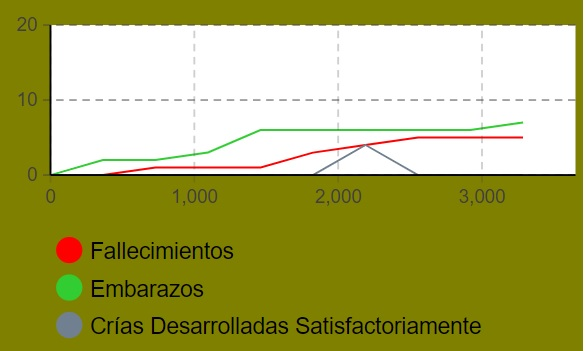
\includegraphics{imagen1}
        \caption{Cantidad de fallecimientos, embarazos y crías en total que se desarrollaron satisfactoriamente en la época de crianza}
        \label{fig:fig1}
    \end{figure}
    \begin{figure}[H]
        \centering
        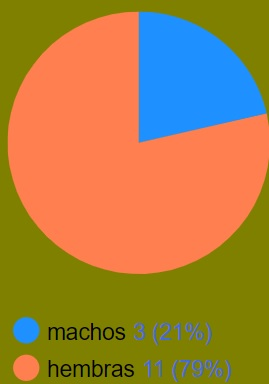
\includegraphics{imagen2}
        \caption{Cantidad de yaguaretés hembras en comparación con cantidad de machos}
        \label{fig:fig2}
        \centering
        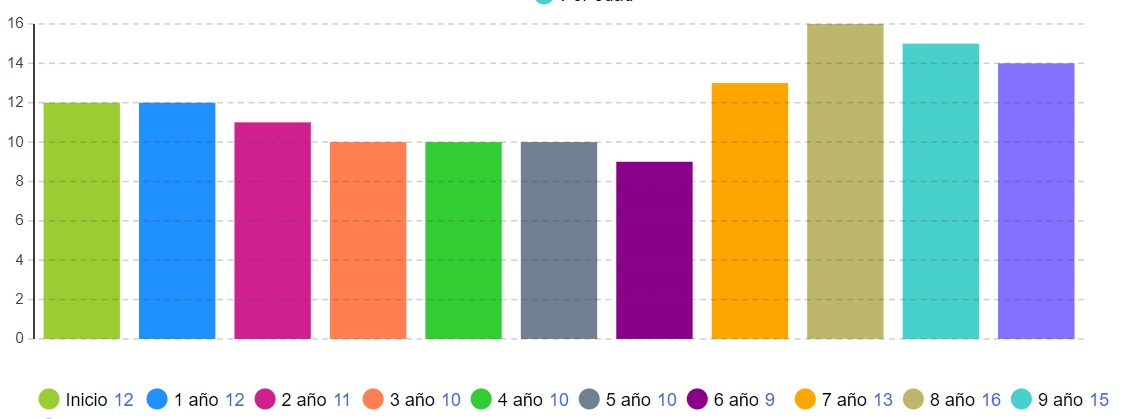
\includegraphics[width=350pt]{imagen4}
        \caption{Cantidad de individuos en el área por año}
        \label{fig:fig4}
    \end{figure}

\section{Verificación y validación del modelo}
    \subsection{Verificación del modelo}
    Hemos comprobado en varias ocasiones el modelo, donde en general han surgido problemas con el movimiento en las
    áreas o distancias entre los individuos.

    Las distribuciones previamente mencionadas corresponden en general a un informe de confianza donde se estudió el
    estilo de vida del yaguareté y en la simulación recreada hemos confirmado de que funcionan correctamente con lo que
    representabamos.

    \subsection{Validación del modelo}
    Casi siempre se notaba que encuentro entre machos era frecuente por lo que esto llevaba a la muerte de muchos de
ellos. Esto en la vida real se puede ver pero no de una manera tan frecuente, en general esta especie busca alejarse de
los problemas entre ellos a menos que se encuentren muy cerca uno de otro.

    Otro punto que encontramos que nos producía diferencias entre los números de poblaciones reales junto con los
resultados que obteníamos era que en general no se producía el apareamiento de manera efectiva.

\section{Generación del modelo final}

Para moldear el modelo de manera que se vea lo más realista posible (con la dificultad que lleva modelar la vida
real de un animal), los arreglos para la verificación del modelo fueron sobretodo por las distancias entre individuos.

Para solucionar las discrepancias de las riñas entre machos, su vida media fue reducida, al igual que la distancia
configurada para que el suceso tome lugar.

Sobre la discrepancia del apareamiento, decidimos aumentar el rango de distancia en el cual los machos podrían encontrar
a una hembra y aparearse. Esto se cambió de manera que no afectara demasiado el apego a la realidad (que no se produzca
a demasiados kilometros de distancia entre un macho y una hembra).

Luego de estos arreglos centrados principalmente en el movimiento de los agentes, el modelo funcionó de manera
satisfactoria, y procedimos a seguir adelante hacia la obtención de los resultados finales.

\section{Determinación de los escenarios para el análisis}

    Decidimos probar 3 escenarios distintos:

    \subsection{Escenario 1: Introducción de misma cantidad de machos y hembras}
        Este escenario contará con una introducción de 6 machos y 6 hembras en una zona con condiciones normales de presas y amenazas. Aquí todas sus características tendrán los valores previamente desarrollados y mencionados.

    \subsection{Escenario 2: Mayor cantidad de machos}
      En este escenario la cantidad de machos es superior, el doble de la cantidad de las hembras. Habrán 8 machos y 4 hembras. Con este escenario se pretende evaluar una zona donde haya una gran disputa del territorio por la cantidad de machos, lo cual no se cree que sería lo ideal, debido a los posibles conflictos que se produzcan entre ellos con los problemas que conllevarían. Tanto la muerte como la salida de la zona bajo estudio de uno de los machos provocarían una disminución de la cantidad de yaguaretés bajo estudio. Por lo que se pretende analizar cuánto nos podría perjudicar en el crecimiento poblacional.

    \subsection{Escenario 3: mayor cantidad de hembras}
      En este escenario, caso contrario del escenario 2, hay más cantidad de hembras que de machos, con lo cual inicialmente se pretende comprobar si la inserción de más individuos de sexo femenino significa que podría nacer más cantidad de crías ayudando al crecimiento poblacional. Si bien la disputa del terreno puede ser menor, también puede ser que la falta de machos influya debido a la falta de encuentro entre ambos sexos. Quizás por tener mucha mayor cantidad de un solo sexo, como también puede suceder que un macho pueda mantener a un grupo de hembras dentro de su territorio con las que se aparea. Esto se podrá comprobar finalmente en las próximas secciones con análisis estadísticos.

    \section{Análisis de sensibilidad}

\subsection{Obtención de datos crudos}

Recopilamos los datos en una planilla de MS Excel y graficamos los promedios de los valores finales de las corridas.

\subsubsection{Escenario 1}
\begin{figure}[H]
    \minipage[t]{0.32\textwidth}
    \includegraphics[width=\linewidth]{esc1/dinamica}
    \caption{Cantidad de fallecimientos, embarazos y crías en total que se desarrollaron satisfactoriamente en la época de crianza}\label{fig:fig1-1}
    \endminipage\hfill
    \minipage[t]{0.32\textwidth}
    \includegraphics[width=\linewidth]{esc1/genero}
    \caption{Cantidad de yaguaretés hembras en comparación con cantidad de machos}\label{fig:fig1-2}
    \endminipage\hfill
    \minipage[t]{0.32\textwidth}
    \includegraphics[width=\linewidth]{esc1/densidad}
    \caption{Cantidad de individuos en el área por año}\label{fig:fig1-3}
    \endminipage
\end{figure}

\subsubsection{Escenario 2}

\begin{figure}[H]
    \minipage[t]{0.32\textwidth}
    \includegraphics[width=\linewidth]{esc2/dinamica}
    \caption{Cantidad de fallecimientos, embarazos y crías en total que se desarrollaron satisfactoriamente en la época de crianza}\label{fig:fig2-1}
    \endminipage\hfill
    \minipage[t]{0.32\textwidth}
    \includegraphics[width=\linewidth]{esc2/genero}
    \caption{Cantidad de yaguaretés hembras en comparación con cantidad de machos}\label{fig:fig2-2}
    \endminipage\hfill
    \minipage[t]{0.32\textwidth}
    \includegraphics[width=\linewidth]{esc2/densidad}
    \caption{Cantidad de individuos en el área por año}\label{fig:fig2-3}
    \endminipage
\end{figure}

\subsubsection{Escenario 3}

\begin{figure}[H]
    \minipage[t]{0.32\textwidth}
    \includegraphics[width=\linewidth]{esc3/dinamica}
    \caption{Cantidad de fallecimientos, embarazos y crías en total que se desarrollaron satisfactoriamente en la época de crianza}\label{fig:fig3-1}
    \endminipage\hfill
    \minipage[t]{0.32\textwidth}
    \includegraphics[width=\linewidth]{esc3/genero}
    \caption{Cantidad de yaguaretés hembras en comparación con cantidad de machos}\label{fig:fig3-2}
    \endminipage\hfill
    \minipage[t]{0.32\textwidth}
    \includegraphics[width=\linewidth]{esc3/densidad}
    \caption{Cantidad de individuos en el área por año}\label{fig:fig3-3}
    \endminipage
\end{figure}

Luego realizamos un análisis estadístico a los resultados de los escenarios que hemos utilizado para llegar a un
estimado de la población que puede llegar a tener en 10 años, en las zonas a las que hemos realizado
el estudio. Esto también nos dará idea su cantidad de mortandad y/o embarazos, junto con la cantidad de crías que
pueden llegar a crecer bajo determinadas condiciones iniciales.

Para poder llegar a estos estimativos utilizaremos el siguiente análisis para así llegar a nuestro objetivo de
verificar la supervivencia del yaguareté en estas zonas elegidas.

        \subsection{Análisis prueba t apareada}
            Para poder realizar una comparación de los distintos escenarios, emplearemos la herramienta de la prueba t apareada con un 95\% de confianza.

            Como puede verse en la figura \ref{fig:esc2-analisis}, la prueba t apareada nos dice que al finalizar la simulación, en el escenario 2 la población tiene una media similar que la del escenario 1, lo que significa que podemos esperar resultados similares en ambas condiciones.

            \begin{figure}[H]
                \centering
                \includegraphics{esc2/analisis}
                \caption{Conclusión de la prueba t apareada comparando el escenario 2 con el 1.}
                \label{fig:esc2-analisis}
            \end{figure}

            El mismo análisis también nos dice que al finalizar la simulación, en el escenario 3 la población tiene una media superior que la del escenario 1 (figura \ref{fig:esc3-analisis}), lo que significa que el escenario 3 presenta mejores condiciones para la supervivencia de la especie.

            \begin{figure}[H]
                \centering
                \includegraphics{esc3/analisis}
                \caption{Conclusión de la prueba t apareada comparando el escenario 3 con el 1.}
                \label{fig:esc3-analisis}
            \end{figure}

            Finalmente, realizamos la comparación del escenario 3 con el escenario 2 (figura \ref{fig:esc3-analisis-2v3}), para la cual el análisis indica que el escenario 3 presenta mejores condiciones que el escenario 2, lo cual coincide con los resultados anteriores.

            \begin{figure}[H]
                \centering
                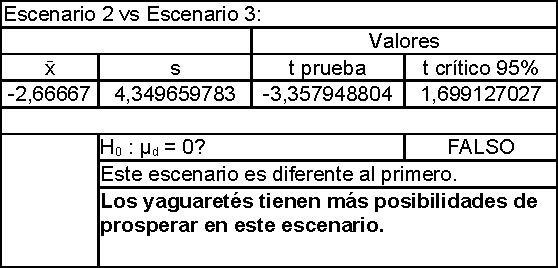
\includegraphics{esc3/analisis-2v3}
                \caption{Conclusión de la prueba t apareada comparando el escenario 3 con el 2.}
                \label{fig:esc3-analisis-2v3}
            \end{figure}

        %\subsection{Intervalos de confianza 2t-muestras modificado}
            
\section{Documentación del modelo, sugerencias y conclusiones}
  Una vez revisados los resultados finales pudimos comprobar que la disposición de los individuos según su sexo es importante. En el caso en el que los machos predominan en una zona, la misma es disputada lo que si bien en nuestro modelo se representa con una mortalidad de uno de los mismos, también podría representar una movilización de uno de los machos fuera de esa zona hacia otra. En la actualidad una problemática que se puede notar en la extinción de la especie en nuestro país (Argentina) es la falta de espacio en donde poder sobrevivir. La destrucción del hogar del yaguareté es un gran factor para la desaparición del mismo. En el caso del modelo nosotros como mencionamos anteriormente suponemos que es una zona en la que no tendría ese problema ya que se representa un ambiente seguro, ya sea un parque nacional o un lugar sin un fácil acceso para el humano.

  Luego hemos visto cómo en estas condiciones que se mencionan, tanto la disposición de una misma cantidad de machos y hembras como una mayor cantidad de machos que de hembras, no han arrojado resultados significativamente diferentes. Por otro lado, en los resultados obtenidos donde predominan las hembras se puede ver una leve mejoría de cantidad de individuos debido a que hay menos disputa de territorios. Estos resultados eran los esperados debido a lo que podíamos ver en la información que habíamos obtenido en nuestra investigación.

  Si bien las hembras también son territoriales, éstas lo hacen para proteger a sus cachorros, además en el territorio de un macho puede haber muchas hembras, lo que permite la reproducción y crecimiento de la población. Por lo tanto en caso de que se debiera introducir una cantidad en una zona de yaguaretés silvestres donde se crea que hay más machos, lo que se podría hacer sería introducir hembras hasta el punto en el que mínimamente se iguale la cantidad de ambos sexos. En el mejor de los casos, se podría insertar en la zona más cantidad de hembras que de machos. Lo ideal sería evitar la inserción de muchos machos debido a la disputa de los territorios, lo cual pudimos comprobar con el modelo de simulación desarrollado y finalmente con el análisis estadístico.

  Como sugerencia, se podría mejorar el modelo en relación con los movimientos de los yaguaretés, lo que quizás se podría revisar un poco más en el código. Sin embargo, consideramos importante que se tenga una actividad continua de rewilding. Esto quiere decir que cada cierto tiempo se vuelvan a introducir nuevos individuos dentro de la zona para que la población de yaguaretés crezca aún más. Ya que como pudimos ver, luego de 10 años los mismos decrecen en números incluso en el mejor de los escenarios vistos. Por esto es que es necesario seguir la regla comprobada en este modelo en el que se inserte mayor cantidad de hembras que de machos.
Esto en conjunto, de evitar introducir mas cantidad de machos, nos permitirá tener una cantidad de yaguaretés adultos en estado salvaje sin contar los probables embarazos o crianzas que se estén dando en ese momento. Otra mejora que se podría hacer sería la inserción de un punto mínimo de individuos de un sexo el cual introduciría un nuevo ejemplar del mismo en base a un mínimo de individuos en el caso de que se necesite.